\documentclass[9pt]{beamer}
\beamertemplatenavigationsymbolsempty
\usetheme{Berlin}

\usepackage{etex, tikz, array, graphics, xspace, relsize, multirow}
\usepackage{ulem}

\input binhex

% For code inclusion
\usepackage{listings}
\lstset{ breaklines=true}
\lstset{escapeinside={<@}{@>}}
\usepackage{algorithm2e}
\usepackage{algorithmic}

% Commands
\newcommand\A{\mathcal{A}}
\newcommand\cc{\mathcal{C}}
\newcommand\codim{\mathrm{codim}}
\newcommand\CP{\mathbb{CP}}
\newcommand\C{\mathbb{C}}
\newcommand\D{\mathrm{D}}
\newcommand\hto{\hookrightarrow}
\newcommand\I{^{-1}}
\newcommand\oo{\mathcal{O}}
\renewcommand\phi{\varphi}
\newcommand\Pj{\mathbb{P}}
\newcommand\pow{\mathcal{P}}
\newcommand\RP{\mathbb{RP}}
\newcommand\rstr[2]{{\left.#1\right|_{#2}}}
\newcommand\R{\mathbb{R}}
\newcommand\V{\mathcal{V}}
\newcommand\H{\mathcal{H}}
\newcommand\set[1]{\{#1\}}
\newcommand\toi{\xrightarrow{\sim}} % category
\newcommand\Z{\mathbb{Z}}


% For drawing
%% Tikz drawing
\usepackage{tikz}
\usetikzlibrary{arrows}
\usetikzlibrary{arrows.meta}
\usepackage{pgfplots}
\usepackage{tikz-3dplot}
\usepackage{tcolorbox}
\usetikzlibrary{matrix,fit,positioning,shapes.geometric,patterns,backgrounds}
\usetikzlibrary{decorations.pathreplacing}
\usetikzlibrary{decorations.markings}
\usetikzlibrary{arrows,calc}
\tikzstyle{bigbox} = [draw=blue!50, thick, rounded corners, rectangle]
\tikzset{
>=stealth'
}
\tikzset{->-/.style={decoration={
  markings,
  mark=at position #1 with {\arrow{>}}},postaction={decorate}}}

%% Software names
\newcommand\topcom{\texttt{TOPCOM}\xspace}
\newcommand\mptopcom{\texttt{MPTOPCOM}\xspace}
\newcommand\mptopcomone{\texttt{MPTOPCOM-1}\xspace}
\newcommand\mts{\texttt{mts}\xspace}
\newcommand\mplrs{\texttt{mplrs}\xspace}
\newcommand\soplex{\texttt{soplex}\xspace}
\newcommand\openmpi{\texttt{OpenMPI}\xspace}
\newcommand\mpi{\texttt{MPI}\xspace}
\newcommand\gfan{\texttt{Gfan}\xspace}
\newcommand\cddlib{\texttt{cddlib}\xspace}
\newcommand\polydb{\texttt{PolyDB}\xspace}
\newcommand\oscar{\texttt{OSCAR}\xspace}

\usepackage{xcolor}
\definecolor{green}{rgb}{0.1,0.59,0.1}
\definecolor{yellow}{rgb}{0.8,0.67,0}
\definecolor{red}{rgb}{0.89,0.1,0.1}
\definecolor{blue}{rgb}{0.1,0.1,0.89}

\usenavigationsymbolstemplate{}

\usepackage{booktabs}
% For software citations
\newcommand{\polymake}{\texttt{po\-ly\-ma\-ke}\xspace}
\newcommand{\polymakejl}{\texttt{Po\-ly\-ma\-ke.jl}\xspace}
\newcommand{\singular}{\texttt{Sin\-gu\-lar}\xspace}
\newcommand\CPP{C\nolinebreak\hspace{-.05em}\raisebox{.4ex}{\relsize{-3}{\textbf{+}}}\nolinebreak\hspace{-.10em}\raisebox{.4ex}{\relsize{-3}{\textbf{+}}}\xspace}

\usepackage{amsmath}
% Newcommands specifically for this article
\newcommand{\eval}{v}               % evaluation function giving switch table
\newcommand{\graph}{\Gamma}         % reverse search graph
\newcommand{\group}{G}              % group acting on point config
\newcommand{\groupElem}{g}          % element of group
\newcommand{\jbound}{\psi}          % bound on the number of elements of set J
\newcommand{\switchTableSize}{\mu}  % index of last non-trivial row in switch table

\newcommand{\pc}{\mathcal P\mathcal C}
\newcommand{\ZZ}{\mathbb Z}
\renewcommand{\AA}{\mathcal A}
\newcommand{\QQ}{\mathbb Q}
\newcommand{\OO}{\mathcal O}
\newcommand{\CC}{\mathbb C}
\newcommand{\PP}{\mathbb P}
\newcommand{\RR}{\mathbb R}
\newcommand{\scalp}[1]{\langle #1 \rangle}
\newcommand{\wt}{\omega}
\newcommand{\cT}{\mathcal T}
\renewcommand{\O}{\mathcal O}
\newcommand{\adm}{\mathcal A(\D, M)}
\newcommand{\blue}[1]{{\usebeamercolor[fg]{palette primary}#1}}

\DeclareMathOperator{\CaDiv}{CaDiv}
\DeclareMathOperator{\conv}{conv}
\DeclareMathOperator{\below}{defect}
\DeclareMathOperator{\vertex}{vertex}
\DeclareMathOperator{\Cox}{Cox}
\DeclareMathOperator{\cl}{cl}
\DeclareMathOperator{\cone}{cone}
\DeclareMathOperator{\Ext}{Ext}
\DeclareMathOperator{\Tor}{Tor}
\DeclareMathOperator{\lcm}{lcm}
\DeclareMathOperator{\Quot}{Quot}
\DeclareMathOperator{\Spec}{Spec}
\DeclareMathOperator{\Sets}{Sets}
\DeclareMathOperator{\relint}{relint}
\DeclareMathOperator{\rk}{rk}
\DeclareMathOperator{\smallestFace}{smallestFace}
\DeclareMathOperator{\Pic}{Pic}
\DeclareMathOperator{\Hom}{Hom}
\DeclareMathOperator{\vol}{vol}
\DeclareMathOperator{\TV}{TV}
\DeclareMathOperator{\tail}{tail}
\DeclareMathOperator{\rep}{rep}
\DeclareMathOperator{\vspan}{span}
\DeclareMathOperator{\canonical}{can}
\DeclareMathOperator{\gkz}{gkz}

\newcommand{\pmsmall}{
\includegraphics[scale=0.03]{pmlogo.png}}
\newcommand{\pmlogo}{
\includegraphics[scale=0.09]{pmlogo.png}}
\newcommand{\pmbluesmall}{\includegraphics[scale=0.03]{pmbluelogo.png}}
\newcommand{\Disjoint}{\mathop{\coprod}}
\newcommand{\Discriminant}{\mathcal{D}}

\theoremstyle{definition}
\newtheorem{remark}{Remark}

\newtheorem{prop}{Proposition}
\newtheorem{defn}{Definition}

\author{Antony Della Vecchia}
\title{The Importance of Symbolic Data Types}
%\newtheorem*{example}{Example}
\institute[]{
Technische Universit\"at Berlin (MaRDI TA1 Computer Algebra)
}
\date{
2022-10-28
}

\logo{
  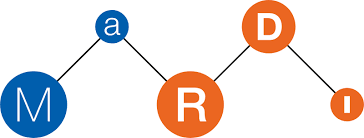
\includegraphics[width=2cm]{images/mardi-logo.png}
}


\newcommand{\surj}{\twoheadrightarrow}
\newcommand{\oursetting}[1]{\textcolor{blue}{#1}}
\usepackage{listings}
\begin{document}
\maketitle
%%%%%%%%%%%%%%%%%%%%%%%%%%%%%%%%%%%%%%%%%%%%%%%%%%%%%%%%%%%%%%%%%%%%%%%%%%%%%%%
%%%%%%%%%%%%%%%%%%%%%%%%%%%%%%%%%%%%%%%%%%%%%%%%%%%%%%%%%%%%%%%%%%%%%%%%%%%%%%%
%%%%%%%%%%%%%%%%%%%%%%%%%%%%%%%%%%%%%%%%%%%%%%%%%%%%%%%%%%%%%%%%%%%%%%%%%%%%%%%

\begin{frame}[fragile]{Expect the Unexpected}
  ``This was unexpected because while I expected numerical error could be possible in the constraints'' . . . `` I did not expect a completely incorrect result''
  \begin{flushright}- Github User
    \end{flushright}
\end{frame}

%%%%%%%%%%%%%%%%%%%%%%%%%%%%%%%%%%%%%%%%%%%%%%%%%%%%%%%%%%%%%%%%%%%%%%%%%%%%%%%
%%%%%%%%%%%%%%%%%%%%%%%%%%%%%%%%%%%%%%%%%%%%%%%%%%%%%%%%%%%%%%%%%%%%%%%%%%%%%%%
%%%%%%%%%%%%%%%%%%%%%%%%%%%%%%%%%%%%%%%%%%%%%%%%%%%%%%%%%%%%%%%%%%%%%%%%%%%%%%%

\begin{frame}[fragile]{Overview}
  \begin{tcolorbox}
    \tableofcontents
  \end{tcolorbox}
\end{frame}
%%%%%%%%%%%%%%%%%%%%%%%%%%%%%%%%%%%%%%%%%%%%%%%%%%%%%%%%%%%%%%%%%%%%%%%%%%%%%%%
%%%%%%%%%%%%%%%%%%%%%%%%%%%%%%%%%%%%%%%%%%%%%%%%%%%%%%%%%%%%%%%%%%%%%%%%%%%%%%%

%%%%%%%%%%%%%%%%%%%%%%%%%%%%%%%%%%%%%%%%%%%%%%%%%%%%%%%%%%%%%%%%%%%%%%%%%%%%%%% 
\section{Convex Hulls}
%%%%%%%%%%%%%%%%%%%%%%%%%%%%%%%%%%%%%%%%%%%%%%%%%%%%%%%%%%%%%%%%%%%%%%%%%%%%%%% 

%%%%%%%%%%%%%%%%%%%%%%%%%%%%%%%%%%%%%%%%%%%%%%%%%%%%%%%%%%%%%%%%%%%%%%%%%%%%%%%
%%%%%%%%%%%%%%%%%%%%%%%%%%%%%%%%%%%%%%%%%%%%%%%%%%%%%%%%%%%%%%%%%%%%%%%%%%%%%%%
%%%%%%%%%%%%%%%%%%%%%%%%%%%%%%%%%%%%%%%%%%%%%%%%%%%%%%%%%%%%%%%%%%%%%%%%%%%%%%%

\begin{frame}[fragile]{Convex Hull Definition}
  \begin{defn}
    A set is $S$ is \emph{convex} if for any two points $p_1, p_2 \in S$ the line
    between them lies entirely in $S$. The \emph{convex hull} of a finite point set
    $V$ is the intersection of all convex sets which contains $V$.
  \end{defn}

  \begin{figure}
    \includegraphics[width=.4\textwidth, height=0.25\textheight]{images/convex-concave}
    \caption{Weisstein, Eric W. "Concave." From MathWorld--A Wolfram Web Resource. \url{mathworld.wolfram.com/Concave.html}}

  \end{figure}
  
\end{frame}
%%%%%%%%%%%%%%%%%%%%%%%%%%%%%%%%%%%%%%%%%%%%%%%%%%%%%%%%%%%%%%%%%%%%%%%%%%%%%%%
%%%%%%%%%%%%%%%%%%%%%%%%%%%%%%%%%%%%%%%%%%%%%%%%%%%%%%%%%%%%%%%%%%%%%%%%%%%%%%%
%%%%%%%%%%%%%%%%%%%%%%%%%%%%%%%%%%%%%%%%%%%%%%%%%%%%%%%%%%%%%%%%%%%%%%%%%%%%%%%

\begin{frame}[fragile]{Convex Hull Descriptions}
  Convex hulls can be described uniquely in multiple ways

  \begin{itemize}
  \item By their set of vertices.
  \item By a system of inequalities.
  \end{itemize}

  These properties make convex hulls computationally ``nice''. That is, they are
  easy for a computer to describe them and there exists algorithms to go between
  these descriptions.
  \begin{figure}
    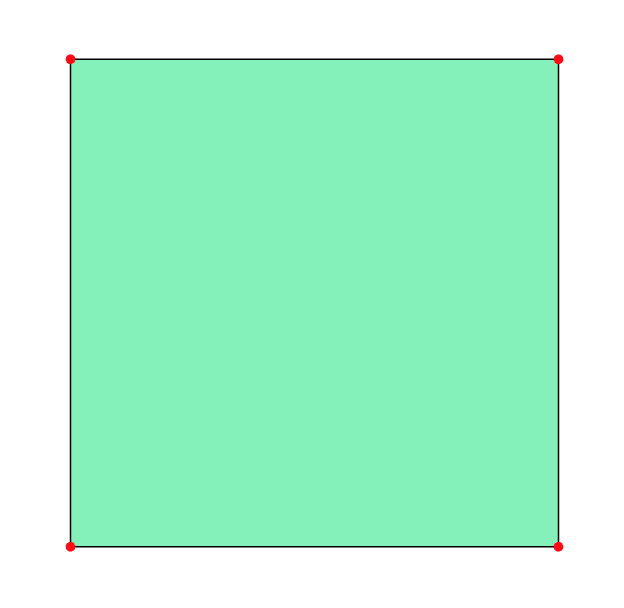
\includegraphics[width=.4\textwidth, height=0.4\textheight]{images/square}
  \end{figure}

\end{frame}
%%%%%%%%%%%%%%%%%%%%%%%%%%%%%%%%%%%%%%%%%%%%%%%%%%%%%%%%%%%%%%%%%%%%%%%%%%%%%%%
%%%%%%%%%%%%%%%%%%%%%%%%%%%%%%%%%%%%%%%%%%%%%%%%%%%%%%%%%%%%%%%%%%%%%%%%%%%%%%%
%%%%%%%%%%%%%%%%%%%%%%%%%%%%%%%%%%%%%%%%%%%%%%%%%%%%%%%%%%%%%%%%%%%%%%%%%%%%%%%

\begin{frame}[fragile]{Where to Find Convex Hulls}
  Convex hulls play a very important role in computational geometry and arise naturally in scientific computations. 

  \begin{itemize}
  \item Optimization over a set of linear constraints (simplex algorithm).
  \item Intersections of bezier curves.
  \item The state space of any quantum system.
  \item Approximations of convex bodies.
  \end{itemize}

  \begin{figure}
    \includegraphics[width=.30\textwidth, height=0.4\textheight]{images/bezier}
  \end{figure}

\end{frame}
%%%%%%%%%%%%%%%%%%%%%%%%%%%%%%%%%%%%%%%%%%%%%%%%%%%%%%%%%%%%%%%%%%%%%%%%%%%%%%%
%%%%%%%%%%%%%%%%%%%%%%%%%%%%%%%%%%%%%%%%%%%%%%%%%%%%%%%%%%%%%%%%%%%%%%%%%%%%%%%
%%%%%%%%%%%%%%%%%%%%%%%%%%%%%%%%%%%%%%%%%%%%%%%%%%%%%%%%%%%%%%%%%%%%%%%%%%%%%%%

%%%%%%%%%%%%%%%%%%%%%%%%%%%%%%%%%%%%%%%%%%%%%%%%%%%%%%%%%%%%%%%%%%%%%%%%%%%%%%%
\section{Convex Hulls Gone Wrong}
%%%%%%%%%%%%%%%%%%%%%%%%%%%%%%%%%%%%%%%%%%%%%%%%%%%%%%%%%%%%%%%%%%%%%%%%%%%%%%%




\begin{frame}[fragile]{A Real World Example}
  The following example was taken from an open github issue from CDDLib and can be found here.
  \url{https://github.com/cddlib/cddlib/issues/67}

  \begin{figure}
    \includegraphics[width=.40\textwidth, height=0.4\textheight]{images/real-example}
  \end{figure}

  \begin{itemize}
  \item The red points were returned from the convex hull computation.
  \item The blue points were missing.
  \item Although finding the right precision may help, it is not apriori clear what that precision is.
  \end{itemize}
  
\end{frame}
%%%%%%%%%%%%%%%%%%%%%%%%%%%%%%%%%%%%%%%%%%%%%%%%%%%%%%%%%%%%%%%%%%%%%%%%%%%%%%%
%%%%%%%%%%%%%%%%%%%%%%%%%%%%%%%%%%%%%%%%%%%%%%%%%%%%%%%%%%%%%%%%%%%%%%%%%%%%%%%
%%%%%%%%%%%%%%%%%%%%%%%%%%%%%%%%%%%%%%%%%%%%%%%%%%%%%%%%%%%%%%%%%%%%%%%%%%%%%%%

\begin{frame}[fragile]{Constructed Example Part 1}
  \begin{defn}
    The \emph{moment curve} $\mu_n \to \mathbb{R}^n$ is defined as
    $\tau \to (\tau, \dots, \tau^n)$. A \emph{cyclic polytope}
    is the convex hull of points on the moment curve.
  \end{defn}
    
  \begin{remark}
    Notice that since any $n + 1$ vertices lie in a distinct supporting
    hyperplane, each facet is an $n$-simplex. 
  
  \end{remark}

  \begin{center}
    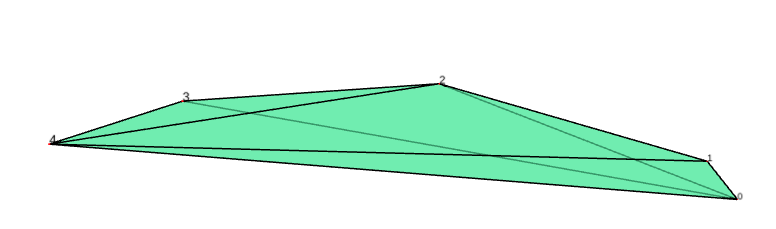
\includegraphics[width=.30\textwidth, height=0.4\textheight]{images/cyclic}
  \end{center}

\end{frame}

%%%%%%%%%%%%%%%%%%%%%%%%%%%%%%%%%%%%%%%%%%%%%%%%%%%%%%%%%%%%%%%%%%%%%%%%%%%%%%%
%%%%%%%%%%%%%%%%%%%%%%%%%%%%%%%%%%%%%%%%%%%%%%%%%%%%%%%%%%%%%%%%%%%%%%%%%%%%%%%
%%%%%%%%%%%%%%%%%%%%%%%%%%%%%%%%%%%%%%%%%%%%%%%%%%%%%%%%%%%%%%%%%%%%%%%%%%%%%%%

\begin{frame}[fragile]{Constructed Example Part 2}
  \includegraphics[width=.90\textwidth, height=0.4\textheight]{images/constructed-1}
\end{frame}

%%%%%%%%%%%%%%%%%%%%%%%%%%%%%%%%%%%%%%%%%%%%%%%%%%%%%%%%%%%%%%%%%%%%%%%%%%%%%%%
%%%%%%%%%%%%%%%%%%%%%%%%%%%%%%%%%%%%%%%%%%%%%%%%%%%%%%%%%%%%%%%%%%%%%%%%%%%%%%%
%%%%%%%%%%%%%%%%%%%%%%%%%%%%%%%%%%%%%%%%%%%%%%%%%%%%%%%%%%%%%%%%%%%%%%%%%%%%%%%

\begin{frame}[fragile]{Constructed Example Part 3}
  \includegraphics[width=.90\textwidth, height=0.9\textheight]{images/constructed-2}

  This code was run in \texttt{polymake}.
\end{frame}



%%%%%%%%%%%%%%%%%%%%%%%%%%%%%%%%%%%%%%%%%%%%%%%%%%%%%%%%%%%%%%%%%%%%%%%%%%%%%%%
%%%%%%%%%%%%%%%%%%%%%%%%%%%%%%%%%%%%%%%%%%%%%%%%%%%%%%%%%%%%%%%%%%%%%%%%%%%%%%%
%%%%%%%%%%%%%%%%%%%%%%%%%%%%%%%%%%%%%%%%%%%%%%%%%%%%%%%%%%%%%%%%%%%%%%%%%%%%%%%


%%%%%%%%%%%%%%%%%%%%%%%%%%%%%%%%%%%%%%%%%%%%%%%%%%%%%%%%%%%%%%%%%%%%%%%%%%%%%%%
\section{Oscar and Data Types}
%%%%%%%%%%%%%%%%%%%%%%%%%%%%%%%%%%%%%%%%%%%%%%%%%%%%%%%%%%%%%%%%%%%%%%%%%%%%%%%

\begin{frame}[fragile]{Exact Computations}
  Possible alternatives to working with floating points would be to consider these
  data types.
  
  \begin{itemize}
  \item rationals
  \item multi precision float (integers, rationals, complex numbers)
  \item arb, acb (arbitrary real ball, arbitrary complex ball)
  \item nmod, nf\_elem, ...
  \item fmpz\_poly, fmpq\_mpoly
  \item ...
  \end{itemize}

  Working with these types is possible within OSCAR, and we are close to releasing
  a version where computing convex hulls over ordered fields (for example finite extensions of $\mathbb{Q}$). 
\end{frame}

%%%%%%%%%%%%%%%%%%%%%%%%%%%%%%%%%%%%%%%%%%%%%%%%%%%%%%%%%%%%%%%%%%%%%%%%%%%%%%%
%%%%%%%%%%%%%%%%%%%%%%%%%%%%%%%%%%%%%%%%%%%%%%%%%%%%%%%%%%%%%%%%%%%%%%%%%%%%%%%
%%%%%%%%%%%%%%%%%%%%%%%%%%%%%%%%%%%%%%%%%%%%%%%%%%%%%%%%%%%%%%%%%%%%%%%%%%%%%%%

\begin{frame}[fragile]{Shift of Perspective on Mathematical Computations}
  \begin{itemize}
    \item The previous slide gives a glimpse into what MaRDI TA1 (Computer Algebra) is concerned with.
    \item The biggest tradeoff is speed ( a lot time goes into multiplication).
    \item The focus turns to finding the combinatorics and storing the data.
    \item Finding a data format has been a first step. (IR)
  \end{itemize}
\end{frame}

%%%%%%%%%%%%%%%%%%%%%%%%%%%%%%%%%%%%%%%%%%%%%%%%%%%%%%%%%%%%%%%%%%%%%%%%%%%%%%%
%%%%%%%%%%%%%%%%%%%%%%%%%%%%%%%%%%%%%%%%%%%%%%%%%%%%%%%%%%%%%%%%%%%%%%%%%%%%%%%
%%%%%%%%%%%%%%%%%%%%%%%%%%%%%%%%%%%%%%%%%%%%%%%%%%%%%%%%%%%%%%%%%%%%%%%%%%%%%%%


\begin{frame}[fragile]{End}
  \begin{center}
    Thank You!
  \end{center}
  \footnotesize{
    \begin{thebibliography}{99} % Beamer does not support BibTeX so references must be inserted manually as below
    \bibitem[polymake]{p1} Ewgenij Gawrilow and Michael Joswig
      \newblock polymake: a framework for analyzing convex polytopes. Polytopes—combinatorics and computation
      \newblock (Oberwolfach, 1997), 43–73, DMV Sem., 29, Birkhäuser, Basel, 2000. MR1785292 (2001f:52033)
      
  \end{thebibliography}
  }
\end{frame}

%%%%%%%%%%%%%%%%%%%%%%%%%%%%%%%%%%%%%%%%%%%%%%%%%%%%%%%%%%%%%%%%%%%%%%%%%%%%%%%
%%%%%%%%%%%%%%%%%%%%%%%%%%%%%%%%%%%%%%%%%%%%%%%%%%%%%%%%%%%%%%%%%%%%%%%%%%%%%%%
%%%%%%%%%%%%%%%%%%%%%%%%%%%%%%%%%%%%%%%%%%%%%%%%%%%%%%%%%%%%%%%%%%%%%%%%%%%%%%%

\end{document}
